\section{Computation of natural frequencies and mode shapes}
\label{sec:computation_of_natural_frequencies_and_mode_shapes}

For the problem at hand, we are dealing with a cantilever beam (see Figure \ref{fig:beam}) with parameters as shown in Table \ref{tab:beam_parameters}.

\begin{figure}[h]
    \centering
    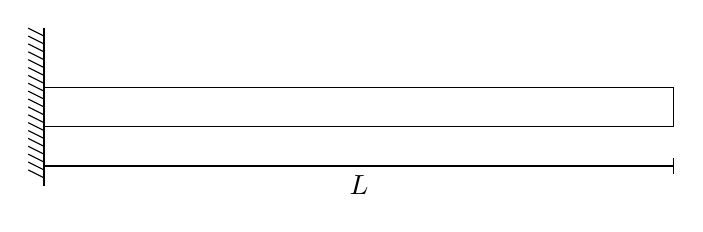
\begin{tikzpicture}[xscale=1, yscale=0.5]

        \draw (0,-0.5) rectangle (8, 0.5);
        \draw[|-|] (0, -1.5) -- (8, -1.5) node[midway, below]{$L$};

        \draw (0, -2) -- (0,  2);

        \foreach \y in {-1.8, -1.6, ..., 1.8}
        \draw (0, \y) -- ++(-0.2, +0.2);

    \end{tikzpicture}
    \caption{Aluminum beam with rectangular cross-section}
    \label{fig:beam}
\end{figure}

\begin{table}[H]
    \centering
    \begin{tabular}{lccc}
        \hline
        Parameter       & Symbol & Unit     & Value  \\
        \hline
        Length          & $L$    & $mm$     & $1200$ \\
        Thickness       & $h$    & $mm$     & $8$    \\
        Width           & $b$    & $mm$     & $40$   \\
        Density         & $\rho$ & $kg/m^3$ & $2700$ \\
        Young's modulus & $E$    & $GPa$    & $68$   \\
        \hline
    \end{tabular}
    \caption{Parameters of the cantilever beam}
    \label{tab:beam_parameters}
\end{table}

For this type of system/structure, considering zero axial-load, the standing wave equation governing its dynamics is:

\begin{equation}
    E I \frac{\partial^4 u}{\partial x^4} = - \rho A \frac{\partial^2 u}{\partial t^2}
\end{equation}

Which, when fully solved, leads to the following formulation of vertical displacement over time $w(x,t)$:

\begin{equation}
    w(x,t) = \left[A\cos(\gamma x) + B\sin(\gamma x) + C\cosh(\gamma x) + D\sinh(\gamma x)\right] \cos(\omega t + \phi)
\end{equation}

Where $\gamma^4 = \frac{m \omega^2}{EJ}$.

By applying the boundary conditions of the cantilever beam, we can find the natural frequencies (and successively also the mode shapes) of the system.
The equations that must be satisfied are:

\begin{equation}
    \begin{cases}
        w(0,t) = 0                                 \\
        \frac{\partial w}{\partial x}(0,t) = 0     \\
        \frac{\partial^2 w}{\partial x^2}(L,t) = 0 \\
        \frac{\partial^3 w}{\partial x^3}(L,t) = 0
    \end{cases}
\end{equation}

By highlighting the four unknowns $A$, $B$, $C$ and $D$, and rearranging the equations in a matrix form, we end up with a linear system as:

\begin{equation}
    [H(\omega)] z
    =
    \begin{bmatrix}
        1               & 0               & 1                & 0                \\
        0               & 1               & 0                & 1                \\
        -\cos(\gamma L) & -\sin(\gamma L) & +\cosh(\gamma L) & +\sinh(\gamma L) \\
        +\sin(\gamma L) & -\cos(\gamma L) & +\sinh(\gamma L) & +\cosh(\gamma L)
    \end{bmatrix}
    \begin{bmatrix}
        A \\
        B \\
        C \\
        D
    \end{bmatrix}
    =
    \begin{bmatrix}
        0 \\
        0 \\
        0 \\
        0
    \end{bmatrix}
    \label{eq:linear_system}
\end{equation}

\subsection{Computation of natural frequencies}
\label{subsec:natural_frequencies}

From theory, we know that the natural frequencies of a system can be computed by solving the following equation:

\begin{equation}
    det[H(\omega_n)] = 0
\end{equation}

Where $H(\omega_n)$ is the matrix as reported in Equation \ref{eq:linear_system} and $\omega_n$ is one of the natural frequencies.

By iterating over a given vector of frequencies, we can compute the value of the determinant of the matrix $H(\omega)$ and find the minimums, which correspond to the natural frequencies of the system.

The result of this computation is shown in Figure \ref{fig:natural_frequencies}.

\begin{figure}[H]
    \centering
    \includegraphics[width=\textwidth]{img/MATLAB/Part_A/H_module.png}
    \caption{Numerical search for natural frequencies of the system. Minimums value of $det[H(\omega)]$ are considered as natural frequencies.}
    \label{fig:natural_frequencies}
\end{figure}

\subsection{Computation of mode shapes}
\label{subsec:mode_shapes}

The mode shapes of the system can be computed again by considering the system of Equations \ref{eq:linear_system}.

In particular, given that to each natural frequency $\omega_n$ corresponds a mode shape, we can compute the mode shapes by solving the linear system for each natural frequency.
However, even if the system is exactly the same, it's important to understand that our goal now is to find the values of $A$, $B$, $C$ and $D$ that satisfy the system of equations, rather that finding the natural frequencies that cancel $H$.

In the end we will have a set of mode shapes, each one corresponding to a natural frequency of the system:

\begin{equation}
    H(\omega_{n, i}) z_i = 0
\end{equation}

By imposing the first component of the solution vector $z_i$ to be $A = 1$, we can find the other components of the solution vector.

\begin{equation}
    [H(\omega_{n, i})] z_i
    \rightarrow
    \hat z_i
    =
    \begin{bmatrix}
        B \\
        C \\
        D
    \end{bmatrix}
    =
    - \begin{bmatrix}
        1               & 0                & 1                \\
        -\sin(\gamma L) & +\cosh(\gamma L) & +\sinh(\gamma L) \\
        -\cos(\gamma L) & +\sinh(\gamma L) & +\cosh(\gamma L)
    \end{bmatrix}^{-1}
    \begin{bmatrix}
        0               \\
        -\cos(\gamma L) \\
        +\sin(\gamma L)
    \end{bmatrix}
    \label{eq:linear_system_for_mode_shapes}
\end{equation}

Once all the mode shapes coefficients ($A = 1$, $B$, $C$ and $D$) are computed, we can plot them with the indication of the associated natural frequency (see Figure \ref{fig:ideal_mode_shapes}).

\begin{figure}[H]
    \begin{minipage}[b]{0.45\textwidth}
        \centering
        \includegraphics[width=0.9\textwidth]{img/MATLAB/Part_A/Mode_shapes/mode_shape_01.png}
    \end{minipage}
    \hfill
    \begin{minipage}[b]{0.45\textwidth}
        \centering
        \includegraphics[width=0.9\textwidth]{img/MATLAB/Part_A/Mode_shapes/mode_shape_02.png}
    \end{minipage}
    \begin{minipage}[b]{0.45\textwidth}
        \centering
        \includegraphics[width=0.9\textwidth]{img/MATLAB/Part_A/Mode_shapes/mode_shape_03.png}
    \end{minipage}
    \hfill
    \begin{minipage}[b]{0.45\textwidth}
        \centering
        \includegraphics[width=0.9\textwidth]{img/MATLAB/Part_A/Mode_shapes/mode_shape_04.png}
    \end{minipage}
    \caption{Computed mode shapes starting from the ideal model of the cantilever beam.}
    \label{fig:ideal_mode_shapes}
\end{figure}
